\documentclass[a4paper, 11pt]{article}
\renewcommand{\baselinestretch}{0.8}
\usepackage[T2A]{fontenc}
\usepackage[utf8]{inputenc}
\usepackage[english, russian]{babel}
\usepackage{multicol}
\usepackage[left=1.5cm,right=2cm,top=0.3cm,bottom=1cm]{geometry}
\usepackage{graphicx,parskip,color} %Вставка картинок правильная
\usepackage{float} %"Плавающие" картинки вроде полезно 
\usepackage{wrapfig} %Обтекание фигур (таблиц, картинок и прочего) хз зачем
\usepackage{vwcol} % столбцы разные епта
\usepackage{paracol} % другие разные стоблцы
\usepackage[format=plain, font=it]{caption}
\usepackage{setspace}
\usepackage{tabularx}
\columnratio{0.33}
\captionsetup[figure]{font=scriptsize}
\newcolumntype{Z}{>{\scriptsize\Centering}X}
\pagestyle {empty}
\usepackage[margin=3em]{geometry}
\begin{document}
\begin{titlepage}
\sffamily
    {\centering
        \vspace*{5em}
        \Large УНИВЕРСИТЕТ ИТМО \par\bigbreak
        \vspace*{3em}
        \large Факультет программной инженерии и компьютерной техники
        \par\bigbreak
        Направление подготовки 09.03.04 Программная инженерия\par\bigbreak
        Дисциплина «Информатика» \par\bigbreak
        \vspace*{2em}
        \Large Отчет \par\bigbreak
        \large По лабораторной работе №6 \par\bigbreak
        «Работа с системой компьютерной верстки TEX» \par\bigbreak
        Вариант 82 \par\bigbreak
    }
    \vspace*{10em}
    \begin{flushright}
    \begin{minipage}{.20\textwidth}
        {\normalsize
        Студент\par\bigbreak
        Рахимов И.И.\par\bigbreak
        Р3119\par\bigbreak
        \vspace*{3em}
        Преподаватель\par\bigbreak
        Рыбаков С.Д.\par\bigbreak
        }
    \end{minipage}
    \end{flushright}
    {\centering
        \vspace*{12em}
        Санкт-Петербург, 2023 г. \par
    }
\end{titlepage}
    \centerline{        КАК УСТРОЕННЫ МЕТАЛЛЫ?}
    \begin{flushright}5\end{flushright}
    \begin{paracol}{2}
        \selectlanguage{russian}
        \begin{figure}[h]
        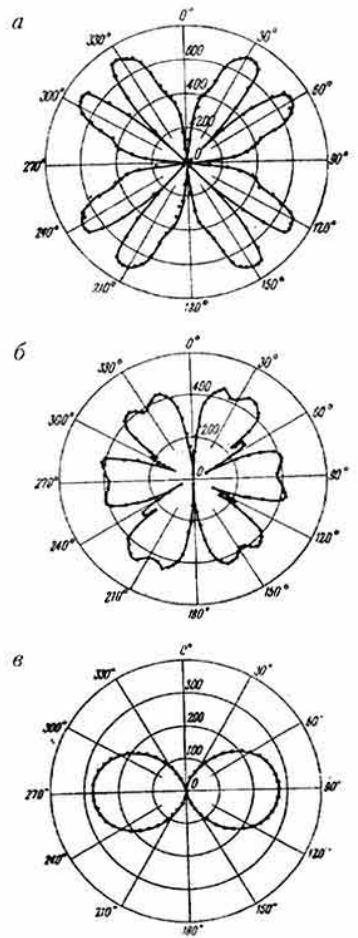
\includegraphics[width=5.8cm, height=16.8cm]{image.png}
        \caption{Изменение сопротивления металла - олова, свинца и таллия соответственно - при помещении его в магнитное поле, (в зависимости от угла между кристаллическими осями и магнитным полем)}
        %\label{fig:mpr}
        \end{figure}
        {\setstretch{0.1}\fontsize{8}{12}\selectfont
        Именно на ней и вокруг этой поверхности находятся электроны, играющие важную роль в свойствах металлов.
        }\\
        \noindent\rule{\columnwidth}{1pt}
        \textbf{\fontsize{13}{2}\selectfont\ Металлы отличаются друг от друга тем, что у них разные поверхности Ферми}\\
        \noindent\rule{\columnwidth}{1pt}
        \setlength{\emergencystretch}{1em}
        {\fontsize{8}{12}\selectfont Прежде чем познакомится с тем, как узнали, каковы поверхности Ферми разных металлов, и какую роль в процессе понимания устройств металлов сыграли работы Илья Михайловича Лифшица и его учеников, посмотрите таблицу. В ней собраны сведения о том, чем похожи и чем отличатся электроны в свободном}
        \\ \\ \\ 
        {\fontsize{6}{12}\selectfont 2 Квант № 2}
        \switchcolumn
        \begin{multicols}{2}
        {\fontsize{8}{2}\selectfont от сил пространстве и в периодическом поле сил ионов кристаллической решетки.\\
        Проблема в устройствах макроскопических, в частности твердых, тел интересовала И.М.Лифшица с самого начала его научной деятельности. Интересы его в большой мере сосредотачивались на решении «обратных» задач. Он неоднократно задумывался}
        \columnbreak
        \\
        {\fontsize{8}{2}\selectfont рассеянию нейтронов кристаллами\textsuperscript{4}. Однако этот метод принцпипально не применим для исследования харакетра движения электронов металла. К счастью, в случае электронов есть важное облегчающее обстоятельство: нас интересуют не все электроны, а лишь те, энергия которых равна энергии Ферми или близка ей. А это значит, что мы должны уметь}
        \end{multicols}
        \begin{tabularx}{\columnwidth}{|Z|Z|}
            \hline
            \multicolumn{2}{|c|}{\fontsize{8}{10}\selectfontЭлектрон}\\ \hline
            в свободном пространстве & в кристалле \\ \hline
            \multicolumn{2}{|c|}{\fontsize{8}{10}\selectfontсостояние характеризуется}\\ \hline
            импульсом (\overrightarrow{\rho}) & квазиимпульсом (\overrightarrow{\rho}) \\ \hline
            \multicolumn{2}{|c|}{\fontsize{8}{10}\selectfontэнергия (\varepsilon)}\\ \hline
            $\varepsilon = \rho^2 / (2m)$ & $\varepsilon = \varepsilon (\overrightarrow{\rho})$ - периодическая функция квазиимпульса \\ \hline
            \multicolumn{2}{|c|}{\fontsize{8}{10}\selectfontскорость (\overrightarrow{\upsilon})}\\ \hline
            $\overrightarrow{\upsilon} = \frac{\overrightarrow{\rho}}{m}$ & $\overrightarrow{\upsilon} = \frac{d \varepsilon(\overrightarrow{\rho})}{d \overrightarrow{\rho}} \neq \frac{\overrightarrow{\rho}}{m}$ \\ \hline
            \multicolumn{2}{|c|}{\fontsize{8}{10}\selectfontуравнение движения}\\ \hline
            изменение импульса в единицу времени равно силе \overrightarrow{F} (закон Ньютона) \[\frac{d \overrightarrow{\rho}}{d t} = \overrightarrow{F},\] \[\frac{d^2 \overrightarrow{r}}{d t^2} = \frac{1}{m} \overrightarrow{F}\] & изменение квазиимпульса в единицу времени равно внешней силе $F^{\textrm{вн}}$ (в $F^{\textrm{вн}}$ не входит переодическая сила ионов кристалла) \[\frac{d \overrightarrow{\rho}}{d t} = \overrightarrow{F},\] \[\frac{d^2x_1}{dt^2} = \sum_{k=1}^{3} \left(\frac{1}{m^2}\right)_a F_{k}^{vn}, \textrm{где}\] \[\left(\frac{1}{m^{2}}\right)_{d} = \frac{\delta^{2}\varepsilon(\overrightarrow{\rho})}{\delta\rho_{2}\delta\rho{3}} \] \\  \hline
            \multicolumn{2}{|c|}{\fontsize{8}{10}\selectfontзакон сохранения энергии и импульса} \\
            \multicolumn{2}{|c|}{\fontsize{8}{10}\selectfont(квазиимпульса) двух электронов}\\ \hline
            \multicolumn{2}{|c|}{\[\varepsilon_{1} + \varepsilon_{2} = \varepsilon_{1}^{`} + \varepsilon_{2}^{`}\]} \\
            \[\overrightarrow{\rho}_{1} + \overrightarrow{\rho}_{2} = \overrightarrow{\rho}_{1}^{`} + \overrightarrow{\rho}_{2}^{`}\] & \[\overrightarrow{\rho}_{1} + \overrightarrow{\rho}_{2} = \overrightarrow{\rho}_{1}^{`} + \overrightarrow{\rho}_{2}^{`} + \overrightarrow{K}, \textrm{где}\] \overrightarrow{K} - один из периодов пространства квазиимпульсов  \\ \hline
        \end{tabularx}
        \begin{multicols}{2}
        {\fontsize{8}{10}\selectfont нельзя ли по экспериментальным данным выяснить, как движутся атомы и электроны в твердом теле. У него есть небольшая заметка «О колебаниях релятивистских частиц в сильных полях». Она опубликована в Докладах Академии наук СССР в 1948 году. (Заметки в Докладах содержат не более четырех страниц.) В заметке выясняется, как по зависимости периода колебаний частицы энергии определить профиль потенциальной ямы, в которой частица совершает периодическое движение. Похоже, это - предтеча работ с решением «обратных» задач. А в 1954 году Илья Михайлович сформулировал алгоритм, позволяющий по тепловым свойствам твердых тел получить сравнительно подробную характеристику колебательного энергетического мпектра твердых тел. Его метод существенно дополняет широко применяемый метод определения колебательного спектра по неупругому} 
        \columnbreak
        \\
        {\fontsize{8}{10}\selectfont определять форму поверхности Ферми (см. (8)) и скорости электронов, имеющих фермиевскую энергию. Как обратил внимание Илья Михайлович, на помощь приходят свойства металлов в магнитном поле при низких температурах. \\
        После первых работ (одну их них я постараюсь схематически изложить) возникло направление в исследованиях металлов, ориентированное на изучение поверхностей Ферми. Все они построены по такому принципу: если поверхность Ферми обладает таким-то свойством, то наблюдается такое-то явление. По идее, должны использоваться подобные работы «в обратном порядке»: наблюдается такое-то явление, значит поверхность}
        \rule{2.5cm}{0.4pt} \\
        {\fontsize{6}{8}\selectfont \sl \textsuperscript{4} Пролетая через кристалл, нейтрон может «качнуть» атомы кристалла. При этом теряет немного энергии и изменяет направление движения. По этим данным определяют, как «качаются» - колеблются атомы кристалла.}
        \end{multicols}
    \end{paracol}
    %\begin{figure}[h]
    %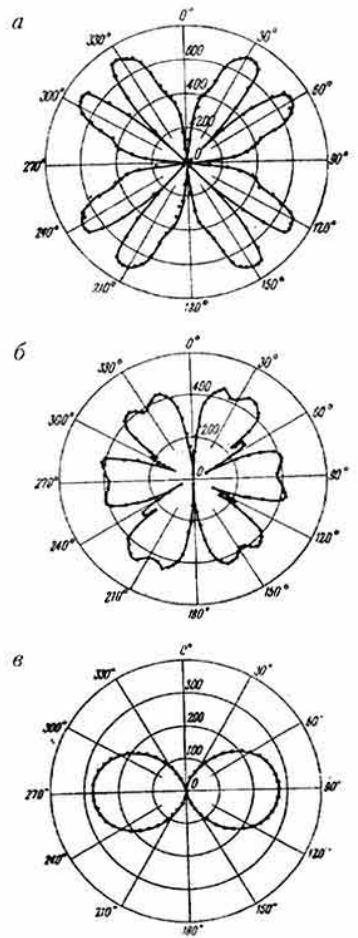
\includegraphics[width=5cm, height=4cm]{image.png}
    %\caption{Диаграмма моментов на участке выбора момента прокатки}
    %\label{fig:mpr}
    %\end{figure}
    % \noindentПривет2

\end{document}